\chapter{Elements of Cartesian Tensor Analysis}

\section{Indicial notation}

Consider $\tenq{u}$ and $\tenq{v}$ which are elements of $E_3$

\[\tenq{u}\cdot\tenq{v}=u_1v_1+u_2v_2+u_3v_3=\sum_{i=1}^3u_iv_i\vc{=}{\footnotemark}{}u_iv_i\]

\footnotetext{Einstein's summation convection}

\section{Range convection}


\begin{itemize}
\item All lower cases, Latin indices (both subscripts and superscripts) have the range 1, 2, 3 or $i, j \in {1, 2, 3}$
\item All lower cases, Greek indices (both subscripts and superscripts) have the range 1, 2 or $\alpha, \beta \in {1, 2}$
\end{itemize}

\begin{enumerate}[label= e.g. \arabic*)]
\item $v_{i}-3$ elements
\item $v_{ij}-3^2$ elements
\item $v_{ijk}-3^3$ elements
\item $v_{\underbrace{ij \cdots k}_{N}}-3^N$ elements
\end{enumerate}

\section{Summation convection}

If in a monomial the same index appears \emph{twice} then summation over this index is implied unless otherwise stated.

\begin{enumerate}[label= e.g. \arabic*)]

\item
\[v_{ii}=v_{11}+v_{22}+v_{33}\]
$v_{ii}\text{ (no sum)}$ either $v_{11}$ or $v_{22}$ or $v_{33}$

\item
\[u_iv_i=u_1v_1+u_2v_2+u_3v_3=u_kv_k=u_jv_j\]

thus repeated indices are \emph{dummy}.

\item
\[a_{ij}x_j=a_{i1}x_1+a_{i2}x_2+a_{i3}x_3\]

indicial equation

\[
a_{ij}x_j=b_i\Longleftrightarrow
\left\{\begin{aligned}
& a_{11}x_1+a_{12}x_2+a_{13}x_3=b_1\\
& a_{21}x_1+a_{22}x_2+a_{23}x_3=b_2\\
& a_{31}x_1+a_{32}x_2+a_{33}x_3=b_3
\end{aligned}\right.
\]

i.e. 3 equations for $i = 1,2,3$

\[a_{ij}x_j=c_{kki}=c_{11i}+c_{22i}+c_{33i}\]

\item NONSENSE

\[a_{i}c_{ji}=b_k\]
(free or non-repeated index on either side is not same)

\[a_{ikk}x_k=c_i\]
(can not have more than two repeated indices)



\end{enumerate}

\paragraph{Rules}\mbox{}\\


\begin{enumerate}[label= (\alph*)]

\item \label{ch2-2-rules-(a)}
The same index cannot appear more than twice \emph{in the same monomial}.

\item \label{ch2-2-rules-(b)}
Free (unrepeated) indices of either side of an indicial equation must agree.
\item
Both free and repeated indicies are \emph{dummy} and may be replaced by other lower case Latin letters subject to restriction \ref{ch2-2-rules-(a)} and \ref{ch2-2-rules-(b)}.

\end{enumerate}

\section{Kronecker delta}

Set of a real numbers, denoted by $\delta_{ij}$ defined as


\[
\delta_{ij}= 
\left\{\begin{aligned} 
& 0 & & \text{if $i \neq j$}\\
& 1 & & \text{if $i=j$}\end{aligned}\right.
\]

\begin{enumerate}[label= e.g. \arabic*)]
\item $\delta_{ii}=3$
\item $\delta_{ii}$ (no sum) $=1$
\item $\delta_{ij}=\delta_{ji}$
\item $\delta_{ij}v_{j}=v_{i}$, $\delta_{ik}v_{kj}=v_{ij}$
\item $\delta_{ij}\delta_{ij}=\delta_{ii}=\delta_{jj}=3$
\item $\delta_{ij}v_{ij}=v_{ii}=v_{jj}=v_{kk}$
\item $\delta_{ik}\delta_{jr}v_{kr}=v_{ij}$
\end{enumerate}

\section{Alternating symbol}

The 27 real numbers $\epsilon_{ijk}$ defined as 

\[\epsilon_{ijk}=1\]

if ($ijk$) are an \emph{even} permutation of the ordered triplet (1 2 3).

\[\epsilon_{ijk}=-1\]

if ($ijk$) are an \emph{odd} permutation of the ordered triplet (1 2 3).


\[\epsilon_{ijk}=0\]

otherwise, i.e. at least two are the same. 

\begin{enumerate}[label= e.g. \arabic*)]
\item $\epsilon_{123}=\epsilon_{231}=\epsilon_{312}=1$
\item $\epsilon_{213}=-1$
\item $\epsilon_{121}=0$
\item $\epsilon_{333}=0$

\item $\epsilon_{ijk}=\epsilon_{jki}=\epsilon_{kij}=-\epsilon_{jik}=-\epsilon_{ikj}=-\epsilon_{kji}$
\item $\epsilon_{ijk}\epsilon_{ijk}=\underbrace{\epsilon_{1jk}\epsilon_{1jk}}_{
\begin{subarray}{l}
  \epsilon_{123}\epsilon_{123} \\
  +\epsilon_{132}\epsilon_{132}=2
  \end{subarray}
}+\epsilon_{2jk}\epsilon_{2jk}+\epsilon_{3jk}\epsilon_{3jk}=6$


\end{enumerate}

\section{Representation of \texorpdfstring{$3\times 3$}{Lg} determinants}

\[
\epsilon_{1jk}v_jw_k 
= \epsilon_{123}v_2w_3+\epsilon_{132}v_3w_2 = v_2w_3-v_3w_2 = 
\begin{vmatrix}
v_2 & v_3 \\ 
w_2 & w_3
\end{vmatrix}
\]

and 

\[
\epsilon_{2jk}v_jw_k 
= \epsilon_{213}v_1w_3+\epsilon_{231}v_3w_1 = -v_1w_3+v_3w_1 = -
\begin{vmatrix}
v_1 & v_3 \\ 
w_1 & w_3
\end{vmatrix}
\]

then 

\begin{equation}
\epsilon_{ijk}u_iv_jw_k=
\begin{vmatrix}
u_1 & u_2 & u_3 \\ 
v_1 & v_2 & v_3 \\ 
w_1 & w_2 & w_3
\end{vmatrix}\tag{$\ast$}\label{eq: 2-6-*}
\end{equation}

\begin{notation}

\[\text{matrix }\mathbf{V}\vc{=}{\footnotemark}{}[V_{ij}]=
\begin{bmatrix}
V_{11} & V_{12} & V_{13} \\ 
V_{21} & V_{22} & V_{23} \\ 
V_{31} & V_{32} & V_{33} 
\end{bmatrix}
\]


\[
\det[V_{ij}]=
\begin{vmatrix}
V_{11} & V_{12} & V_{13} \\ 
V_{21} & V_{22} & V_{23} \\ 
V_{31} & V_{32} & V_{33}  
\end{vmatrix}=\det\tenq{V}
\]

\end{notation}

\footnotetext{In here, we use $\tenq{V}$ rather than $\mathbf{V}$ for readability, but in writing, we always use $\mathbf{V}$ to represent tensor. Usually (but not always), the uppercase mean the second order tensor, lowercase mean the first order tensor.}


\begin{claim}\mbox{}\\

\begin{equation}
\epsilon_{ijk}\epsilon_{pqr}\det\tenq{V} =
\begin{vmatrix}
V_{ip} & V_{iq} & V_{ir} \\ 
V_{jp} & V_{jq} & V_{jr} \\ 
V_{kp} & V_{kq} & V_{kr}  
\end{vmatrix}\tag{$\ast\ast$}\label{eq: 2-6-**}
\end{equation}

Note the following properties

\[
\det\tenq{V} 
\underset{\begin{subarray}{l}
  \text{from } \eqref{eq: 2-6-*}\\
  \text{replace} \\
  u_{i} \rightarrow V_{1i} \\
  v_{j} \rightarrow V_{2j} \\
  w_{k} \rightarrow V_{3k}
  \end{subarray}}{=}
\epsilon_{ijk}V_{1i}V_{2j}V_{3k} \underset{\text{transpose of }\det\tenq{V}}{=} \epsilon_{ijk}V_{i1}V_{j2}V_{k3}
\]

Also 

\[\epsilon_{pqr}\det\tenq{V}=\epsilon_{ijk}V_{pi}V_{qj}V_{rk}=\epsilon_{ijk}V_{ip}V_{jq}V_{kr}\]

(take care of the permutation of rows or columns of $\det\tenq{V}$)


\begin{align*}
\epsilon_{pqr}\epsilon_{pqr}\det\tenq{V}
&=\epsilon_{ijk}\epsilon_{pqr}V_{ip}V_{jq}V_{kr} \\
\Aboxed{\det\tenq{V}&=\frac{1}{6}\epsilon_{ijk}\epsilon_{pqr}V_{ip}V_{jq}V_{kr}}
\end{align*}


\[\epsilon_{ijk}\epsilon_{pqr}\det\tenq{1}\vc{=}{\eqref{eq: 2-6-**}}{}
\begin{vmatrix}
\delta_{ip} & \delta_{iq} & \delta_{ir} \\ 
\delta_{jp} & \delta_{jq} & \delta_{jr} \\ 
\delta_{kp} & \delta_{kq} & \delta_{kr}  
\end{vmatrix}
\]

where $\tenq{1}=$ identity matrix $=[\delta_{ij}]$


\[\vc{\Rightarrow}{i=p}{}\boxed{\epsilon_{ijk}\epsilon_{iqr}=\delta_{jq}=\delta_{kr}-\delta_{jr}\delta_{kq}}\text{ (proof: Homework)}\]

if $j=q$ further

\[\epsilon_{ijk}=\epsilon_{ijr}=\delta_{jj}\delta_{kr}-\delta_{jr}\delta_{kj}=3\delta_{kr}-\delta_{kr}=2\delta_{kr}\]


\end{claim}

\section{Connection with vector algebra}

Consider vectors $\tenq{u}$, $\tenq{v}$, and $\tenq{w}$ in $E_3$

dot product $\tenq{v}\cdot\tenq{u}$


\[\tenq{v}\cdot\tenq{u}=\abs{\tenq{v}}\abs{\tenq{u}}\cos\theta\]

cross product $\tenq{v}\wedge\tenq{u}\phantom{-}(\tenq{v}\times\tenq{u})$


\[\abs{\tenq{v}\wedge\tenq{u}}=\abs{\tenq{v}}\abs{\tenq{u}}\sin\theta\]

\begin{figure}[H]
\centering
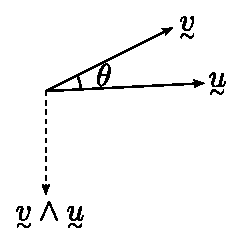
\includegraphics[scale=1.0]{2-7-1.eps}
\caption{Direction of cross product}
\label{Direction of cross product-2-7-1}
\end{figure}

or in determinant form

\begin{equation}
\tenq{v}\wedge\tenq{u}
=
\begin{vmatrix}
\tenq{e}_1 & \tenq{e}_2 & \tenq{e}_3 \\ 
v_1 & v_2 & v_3 \\ 
u_1 & u_2 & u_3
\end{vmatrix}
=
\tenq{e}_1
\begin{vmatrix}
v_2 & v_3 \\ 
u_2 & u_3
\end{vmatrix}
-
\tenq{e}_2
\begin{vmatrix}
v_1 & v_3 \\ 
u_1 & u_3
\end{vmatrix}
+
\tenq{e}_3
\begin{vmatrix}
v_1 & v_2 \\ 
u_1 & u_2
\end{vmatrix}\tag{1}\label{eq: 2-6-(1)}
\end{equation}

Let $X = \left\{ {0;\tenq{e}_1,\tenq{e}_2,\tenq{e}_3} \right\}$ be a rectangular Cartesian coordinate frame with origin $O$ and with unit vector $\tenq{e}_i$.

\begin{framed}
$\mathscr{F}$: the class of all frames\\
$\mathscr{F}_{+}$: the class of all such frames that are also right-handed
\end{framed}

\paragraph{Properties of $\mathscr{F}$ and $\mathscr{F}_+$}\mbox{}\\

if $X \in \mathscr{F} \Rightarrow  \tenq[1]{e}_i \cdot \tenq[1]{e}_j = \delta_{ij}$\\
if $X \in \mathscr{F}_{+} \Rightarrow  \tenq[1]{e}_i \cdot \tenq[1]{e}_j = \delta_{ij}$ and $\left(\tenq[1]{e}_1 \wedge \tenq[1]{e}_2 \right) \cdot \tenq[1]{e}_3 = +1$\\

Let $X\in\mathscr{F}_+$, then the three real numbers defined as
\[u_i^X=\tenq{u}\cdot\tenq{e}_i^X\]

scalar components of vector $\tenq{u}$ on $X$

\begin{note}
No need to put $X$ to the superscript of $\tenq{u}$.
\end{note}

\[\tenq{u}=u_i\tenq{e}_i=u_1\tenq{e}_1+u_2\tenq{e}_2+u_3\tenq{e}_3\]

\begin{align*}
\tenq{u}\cdot\tenq{v}
&= \left(u_i\tenq{e}_i\right)\cdot\left(v_k\tenq{e}_k\right) = u_iv_k\tenq{e}_i\cdot\tenq{e}_k = u_iv_k\delta_{ik} \\
&= u_iv_i=u_kv_k
\end{align*}

\[\therefore\boxed{\tenq{u}\cdot\tenq{v}=u_iv_i}\]

%\begin{align*}
%\Aboxed{\tenq{v}\wedge\tenq{u}
%&\vc{=}{\eqref{eq: 2-6-(1)}}{\eqref{eq: 2-6-*}}\epsilon_{ijk}\tenq{e}_iv_ju_k} \\
%&= \left( \epsilon_{ijk}v_ju_k\right)\tenq{e}_i = \left(\tenq{v}\wedge\tenq{u}\right)_i\tenq{e}_i
%\end{align*}

\begin{equation}
\left.\begin{aligned}
\Aboxed{\tenq{v}\wedge\tenq{u}
&\vc{=}{\eqref{eq: 2-6-(1)}}{\eqref{eq: 2-6-*}}\epsilon_{ijk}\tenq{e}_iv_ju_k} \\
&= \left( \epsilon_{ijk}v_ju_k\right)\tenq{e}_i = \left(\tenq{v}\wedge\tenq{u}\right)_i\tenq{e}_i
\end{aligned}\right. \tag{2}\label{eq: 2-6-(2)}
\end{equation}

\begin{equation}
\therefore\boxed{\left(\tenq{v}\wedge\tenq{u}\right)_i=\epsilon_{ijk}v_ju_k} \tag{3}\label{eq: 2-6-(3)}
\end{equation}

\begin{note}
The expression of equations must be consistent, either in vector form (as \eqref{eq: 2-6-(2)}) or in indicial form (as \eqref{eq: 2-6-(3)}).
\end{note}

\begin{align*}
\left(\tenq{u}\wedge\tenq{v}\right)\cdot\tenq{w}
&= \left(\epsilon_{ijk}u_jv_k\tenq{e}_i\right)\cdot\left(w_l\tenq{e}_l\right) = \epsilon_{ijk}u_jv_kw_l\underbrace{\left(\tenq{e}_{i}\cdot\tenq{e}_l\right)}_{\delta_{il}} \\
&= \epsilon_{ijk}w_iu_jv_k
\end{align*}

If we start with indicial form

\begin{align*}
\left(\tenq{u}\wedge\tenq{v}\right)\cdot\tenq{w}
&= \left(\tenq{u}\wedge\tenq{v}\right)_kw_k = \epsilon_{kij}u_iv_jw_k = \epsilon_{ijk}u_iv_jw_k
\end{align*}

\begin{example}{$\tenq{a}$ and $\tenq{b}$ are any vectors in $E_3$, show that $\left(\tenq{a}\wedge\tenq{b}\right)\cdot\left(\tenq{a}\wedge\tenq{b}\right)+\left(\tenq{a}\cdot\tenq{b}\right)^2=\abs{\tenq{a}}^2\abs{\tenq{b}}^2$.}

\begin{solution}

\begin{align*}
&\left(\tenq{a}\wedge\tenq{b}\right)\cdot\left(\tenq{a}\wedge\tenq{b}\right)+\left(\tenq{a}\cdot\tenq{b}\right)^2 \\
=& \epsilon_{ijk}a_jb_k\epsilon_{ilm}a_lb_m+\left(a_jb_j\right)\left(a_kb_k\right)\\
=& \epsilon_{ijk}\epsilon_{ilm}a_jb_ka_lb_m+a_jb_ja_kb_k \\
=& \left(\delta_{jl}\delta_{km}-\delta_{jm}\delta_{kl}\right)a_jb_ka_lb_m+a_jb_ja_kb_k \\
=& a_jb_ka_jb_k-\cancel{a_jb_ka_kb_j} + \cancel{a_jb_ja_kb_k}\\
=& \abs{\tenq{a}}^2+\abs{\tenq{b}}^2
\end{align*}

\end{solution}

\end{example}

\begin{example}{Show that }

\[
\left(\tenq{a}\wedge\tenq{b}\right)\cdot\left(\tenq{c}\wedge\tenq{d}\right)=
\begin{vmatrix}
\tenq{a}\cdot\tenq{c} & \tenq{b}\cdot\tenq{c} \\ 
\tenq{a}\cdot\tenq{d} & \tenq{b}\cdot\tenq{d}
\end{vmatrix}
\]

\begin{solution}

\begin{align*}
\left(\tenq{a}\wedge\tenq{b}\right)\cdot\left(\tenq{c}\wedge\tenq{d}\right) 
&= \epsilon_{ijk}a_jb_k\epsilon_{ilm}c_ld_m \\
&= \epsilon_{ijk}\epsilon_{ilm}a_jb_kc_ld_m\\
&= \left(\delta_{jl}\delta_{km}-\delta_{jm}\delta_{kl}\right)a_jb_kc_ld_m \\
&= a_jc_jb_kd_k - a_jd_jb_kc_k \\
&= \left(\tenq{a}\cdot\tenq{c}\right)\left(\tenq{b}\cdot\tenq{d}\right)-\left(\tenq{a}\cdot\tenq{d}\right)\left(\tenq{b}\cdot\tenq{c}\right)\\
&= 
\begin{vmatrix}
\tenq{a}\cdot\tenq{c} & \tenq{b}\cdot\tenq{c} \\ 
\tenq{a}\cdot\tenq{d} & \tenq{b}\cdot\tenq{d}
\end{vmatrix}
\end{align*}

\end{solution}

\end{example}



